\newpage
\section{Testing and Comparison}\label{sec:comparison}
After the neural network has been trained with the synthetic data, as described in section \ref{sec:algorithm}, it can be tested on synthetic data, where the decomposition is known by construction, as well as on real world data. To compare the decompositions of real world data, another algorithm is needed for benchmarking, which calculates the decomposition of an arbitrary positive semidefinite matrix $M$ into a low rank, symmetric and positive-semidefinite matrix $L_0$ plus a sparse matrix $S_0$:
\begin{align}
 M = L_0 + S_0.
\end{align}
With \textit{Principal  Component  Pursuit} (PCP), there exists an algorithm, which, under some suitable assumptions, calculates the decomposition exactly via singular value decomposition (SVD) \cite{candes2009robust}. The assumptions and the main ideas of this algorithm is presented in the first subsection. In the second subsection the results of the decomposition of portfolio correlation matrices via the AI algorithm Denise with the results of the Principal Component  Pursuit algorithm.

\subsection{The Minimization Problem solved by PCP}\label{sec:pcpproblem}
Let $M$ be a given element of $\mathbb R^{n_1\times n_2}$. $\norm \cdot_*$ denotes the nuclear norm, i.e. the sum over the singular values of a matrix $\norm M_* \defeq \sum_i \sigma_i(M)$. $\norm \cdot_1$ is the well known $\ell_1$ norm $\norm M_1 = \sum_{ij} \abs{M_{ij}}$. The PCP algorithm solves the convex optimazation problem
\begin{align}
\label{pcpoptproblem}
 \mathrm{minimize} \quad \norm L_* + \norm S_1, \quad \text{where } L+S=M
\end{align}
exactly, if the the low-rank component $L_0$ fulfills a \q{incoherence} condition, and that the sparse component is \q{reasonably sparse}. The meaning of this \q{incoherence} condition for $L_0$ and the \q{reasonable} sparsity of $S_0$ is explained in \cite[subsection 1.3]{candes2009robust}. We summarize the main points real for quadratic matrices:
\par
\begin{enumerate}[label=(\roman*),ref=(\roman*)]
 \item \label{incoherencecond} Let $U\Sigma V^\top$ the singular singular value decomposition of $L_0 \in R^{n\times n}$ with rank $k\ge n$, i.e.
\begin{align}
 L_0 = U\Sigma V^\top = \sum_{i=1}^k \sigma_i u_i v_i^\top,
\end{align}
where $U=(u_1,\dots,u_k),V=(v_1,\dots,v_k) \in \mathrm{O}(n)$, $\Sigma=\diag{\sigma_1,\dots,\sigma_r,0,\dots,0} \in \mathbb R^{n\times n}$. $\sigma_1,\dots,\sigma_k$ are the singular values and $u_i$ and $v_i$, $i=1,\dots,k$, are the left-singular and right-singular vectors for $\sigma_i$, respectively. Then the matrix $L_0$ is called incoherent, with parameter $\mu$, if
\begin{align}
 \max_i \norm{U e_i}^2 \ge \dfrac{\mu k}{n^2},\quad  \max_i \norm{V e_i}^2 \ge \dfrac{\mu k}{n^2}, \quad \norm{UV^\top}_\infty \ge \dfrac{\sqrt{\mu k}}{n}.
\end{align}
$e_i$ are the canonical basis vectors of $\mathbb R^n$. 
 \item \label{uniformlysparse} The positions of the nonzero elements of the sparsity matrix are selected uniformly random.
\end{enumerate}
If \ref{incoherencecond} is fulfilled, the matrix $L_0$ is considered as not sparse. With \ref{uniformlysparse} we try to prevent, that the nonzero elements are only in one, or few columns of the sparsity matrix. For example if the entries of $S_0$ except the first column are all zero, and the first column of $S_0$ is the negative of the first column of $L_0$, then it is impossible to recover the low rank component and sparse component exactly. To avoid, such variety of possibilities for the decomposition 
\ref{uniformlysparse} is a reasonable assumption.

\subsection{PCP Algorithm}\label{sec:pcpalgorithm}
\label{sec:PCP}
In this subsection, a brief description of the PCP algorithm, which we use for comparison with Denise, is given. There are different strategies to solve the problem \eqref{pcpoptproblem} numerically. As described in \cite{candes2009robust}, we consider an \textit{augmented Lagrange multiplier}. This is why Candes et al. named this method the ALM method. \eqref{pcpoptproblem} is equivalent to the minimization of the following \textit{augmented Lagrangian}
\begin{align}
 \mathcal L(L,S,Y) = \norm L_* + \lambda \norm S_1 + \langle Y, M -L - S \rangle + \dfrac{\mu}{2} \norm{M - L - S}_F^2.
\end{align}
Here $\langle \cdot, \cdot \rangle$ is defined as 
%$\langle A , B \rangle = \trace{A^\top B}$
$\langle A , B \rangle = \trace{A^\top B}$
, with real quadratic matrices $A,B$. $\norm \cdot_F$ is the Frobenius norm. One can show, that
\begin{alignat}{2}
 &\arg \min_S \mathcal L(L,S,Y) &&= \mathcal S_{\lambda \mu}(M-L+ \mu^{-1} Y), \\
 &\arg \min_L \mathcal L(L,S,Y) &&= \mathcal D_\mu (M-S-\mu^{-1} Y),
\end{alignat}
where $\mathcal S_\tau : \mathbb R^{n \times n} \to \mathbb R^{n \times n}: (X_{ij})_{ij} \mapsto (\sgn{X_{ij}} \max \left( \abs{X_{ij}} - \tau,0 \right))_{ij}$, is the extension of the shrinkage operator in $\mathbb R$ to $\mathbb R^{n \times n}$. $\mathcal D_\tau (X)$ is defined as $\mathcal D_\tau (X) = U \mathcal S_\tau (\Sigma) V^\top$, where $U \Sigma V^\top$ is the SVD of $X$. Hence, the following algorithm, taken from \cite[29]{candes2009robust}, is productive
\begin{enumerate}
 \item \textbf{Initialize}: $\mathrm S_0 = Y_0 = 0,\mu >0$.
 \item \textbf{While} not converged \textbf{do}
    \begin{subequations}
    \begin{alignat}{2}
     &L_{k+1} &&= \mathcal D_\mu(M-S_k-\mu^{-1} Y_k) \\
     &S_{k+1} &&= \mathcal S_{\lambda \mu}(M-L_{k+1} +\mu^{-1} Y_k) \\
     &Y_{k+1} &&= Y_k + \mu(M-L_{k+1} - S_{k+1})
    \end{alignat}
    \end{subequations}
 \item \textbf{Return}: L,S.
\end{enumerate}
With the calculations of the second step, it is avoided to solve a sequence of convex programs. To archieve good relativ accuracy, only a few iteration steps are neccessary \cite[section 3]{candes2009robust}.

\subsection{Evaluation of trained Denise on Financial Data}
To get a first impression of Denise performance on real-world data, we apply Denise on a set of $10$-by-$10$ correlation matrices of ten stocks out of DAX 30, namely Allianz, BASF, Bayer, Beiersdorf, BMW, Continental, Siemens, Merck, Daimler, VW. As a data basis, we exploit the price data of the aforementioned stocks from the last 2 years, starting from January 15th in 2021. The empirical correlation matrices are determined retrospectively with an offset of one day, while the correlations in time step $n$ are calculated based on closing prices within the last 35 days. In the end, we obtain 472 correlation matrices $\mathbf{R}^{(n)}, n = 1, 2, ... , 472 $ for further numerical tests by this approach.
\par
The stock prices required to calculate the empirical correlation matrices are downloaded from \textit{Yahoo! Finance} and then transferred into a CSV file. This CSV file is imported into \textit{Jupyter Notebook} and the price data is stored in vectors $X^{(i)}, i = 1, ... , 10$, beginning with the latest value, in order to calculate the empirical correlation matrices $\mathbf{R}^{(n)}, n = 1, 2, ... , 472 $ according to 
\begin{align}
\mathbf{R}_{i,j}^{(n)} = \frac{\sum_{k=n}^{n+N-1} (X_{k}^{(i)} - \bar{X}^{(i)}) (X_{k}^{(j)} - \bar{X}^{(j)})}{\sqrt{\sum_{k=n}^{n+N-1} (X_{k}^{(i)} - \bar{X}^{(i)})^{2} \sum_{k=n}^{n+N-1}(X_{k}^{(j)} - \bar{X}^{(j)})^{2}}},
\end{align}
where $X_{k}^{(i)}$ is the price of the $i$-th stock at the end of the $k$-th trading day and $N$ the total number of analyzed trading days, within the relevant time period.

\subsection{Portfolio Correlations from DAX 30 with PCP and Denise}
For test purposes we applied the PCP algorithm on 472 empirical correlation matrices of the ten DAX 30 companies, mentioned before. Due to our approach in calculating the different correlation matrices, their structure changes quite slowly. Hence, we concentrate our investigations only on 10 matrices with equidistant time steps.
\par
We train the neural network on a synthetic data set of 1000000 $10\times 10$-matrices of rank three. Training and validation loss are illustrated in Fig. \ref{fig:finance_training}. Figure \ref{fig:finance_sparsity} shows the training and validation sparsity over the epochs. Unfortunately, the reached sparsity of density is not much higher than $\sim 2\%$. The sparsity, that is obtained in the orignal article, is around $\sim 99 \%$ for the finacial data sets \cite[Table 2.]{herrera2020denise}. This is a strong hint, that there is still improvement potential for our neural network. A small training set, aswell as a unsuitable architecture, could responsible that our neural network is not able to reduce the correlation in the data on three main components. The comparison of the RPCA decomposition of the correlations matrices into rank $3$ matrix $L$ and sparse $S$ for both methods is shown in Fig. \ref{fig:compfinance}. Representatively, we have choosen only one decomposition, because the color plots of the ten matrices are quite similar. This simularity allows us to restrict further investigations  concerning the attributes of the decompositions on only one single matrix. As one can see, the decomposition obtained from our neural network suffers significant outliers on the diagonal elements in $L$ as well as $S$, which is not apparent in the PCP decomposition. One explanation for the occurence of the outliers on the diagonal can be the structure of the traning matrices. The normalization of the correlation matrices causes, that the diagonal elements are all set to $1$. Since this particular property is missing in the training data, the network could not process the diagonal elements accurately. Due to this outlier not much structure is visible in $L$ obtained from the neural network. However, apart from the diagonal elements the $S$-matrices of both methods seem to agree to some approximation (respecting the corresponding color code). As a metric, to measure how well the two algorithms agree, we determine the relative errors $\epsilon_\text{rel} (S_\text{PCP}, S_\text{NN}),\, \epsilon_\text{rel} (L_\text{PCP}, L_\text{NN})$ as the relative $l_2$-distance
\begin{align}
\epsilon_\text{rel}(A,B) = \frac{\Vert A - B \Vert_{l_2}}{\Vert A \Vert_{l_2}}
\end{align}
between $S_\text{PCP}, S_\text{NN}$, respectively between $L_\text{PCP}, L_\text{NN}$ (the PCP-, respectively neural-network-prediction for $S$ and $L$):
\begin{align}
\epsilon_\text{rel}(S_\text{PCP},S_\text{NN}) = 3,234\,, \quad  \epsilon_\text{rel}(L_\text{PCP},L_\text{NN}) = 0,909 \,.
\end{align}
The running time for the neural network calculation of the RPCA is $0,0197$ seconds. The PCP algorithm needed $0,131$ seconds. Hence, the neural network approach is approximately an order of magnitude faster.
\begin{figure}
	\centering
	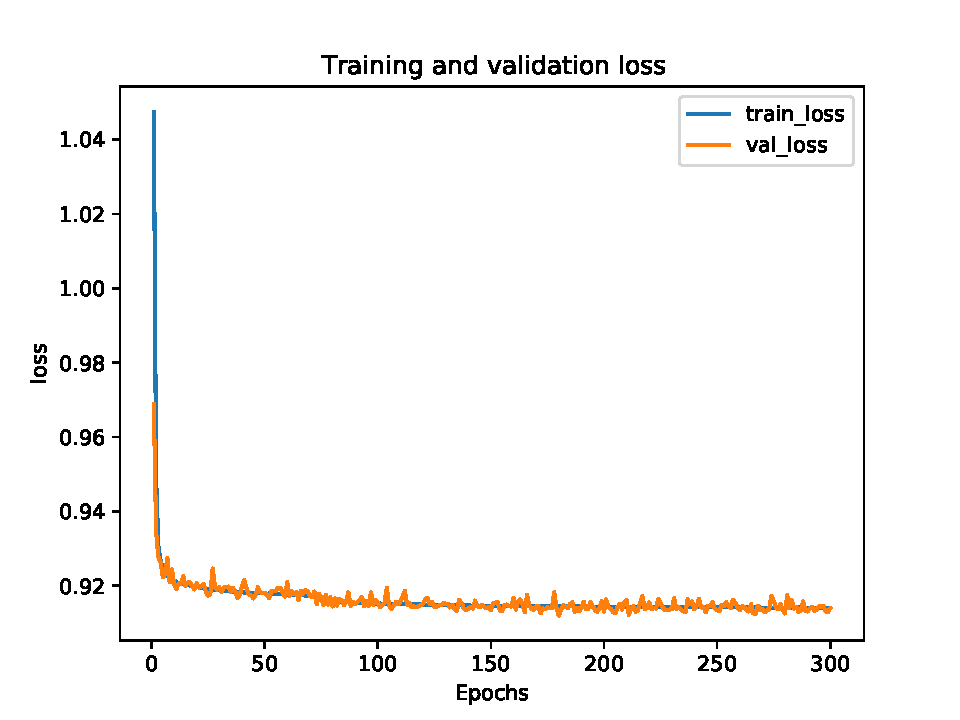
\includegraphics[width=0.9\textwidth]{fig/loss_finance.pdf}
	\caption{Training and validation loss of the network training for finance data.}
	\label{fig:finance_training}
\end{figure}
\begin{figure}
	\centering
	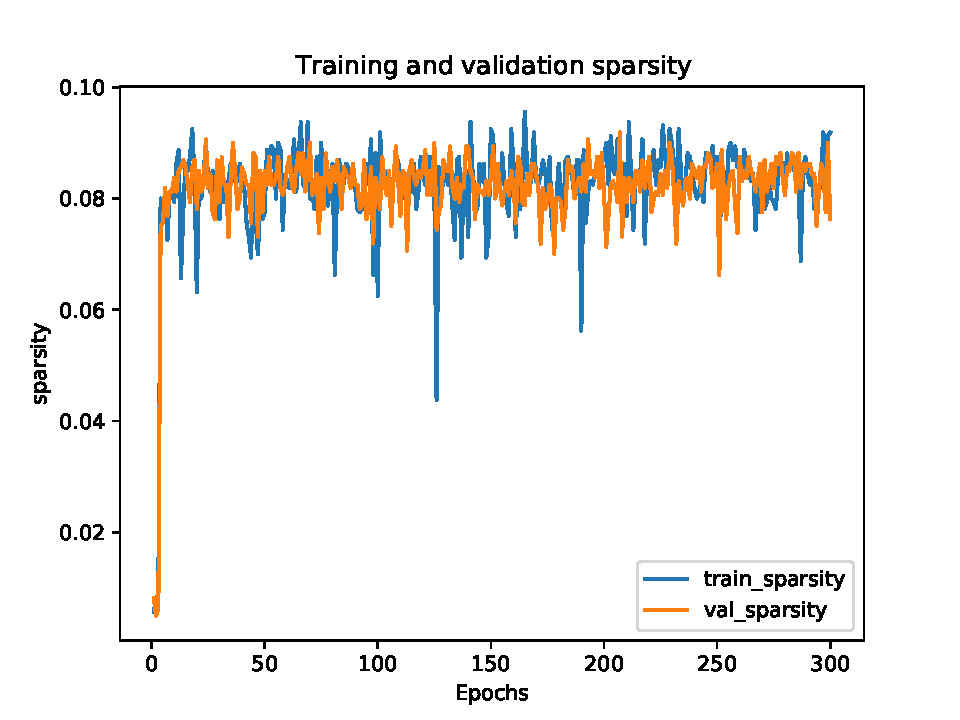
\includegraphics[width=0.9\textwidth]{fig/sparsity_finance.pdf}
	\caption{Training and validation sparsity evolution over the epochs.}
	\label{fig:finance_sparsity}
\end{figure}
\begin{figure}
	\centering
	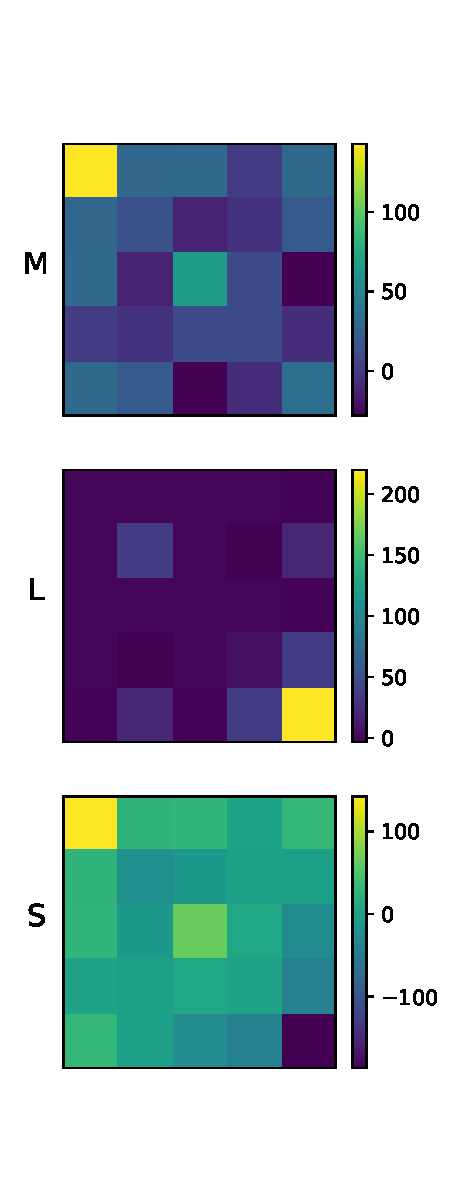
\includegraphics[width=0.48\textwidth]{fig/denise_output_finance.pdf}
	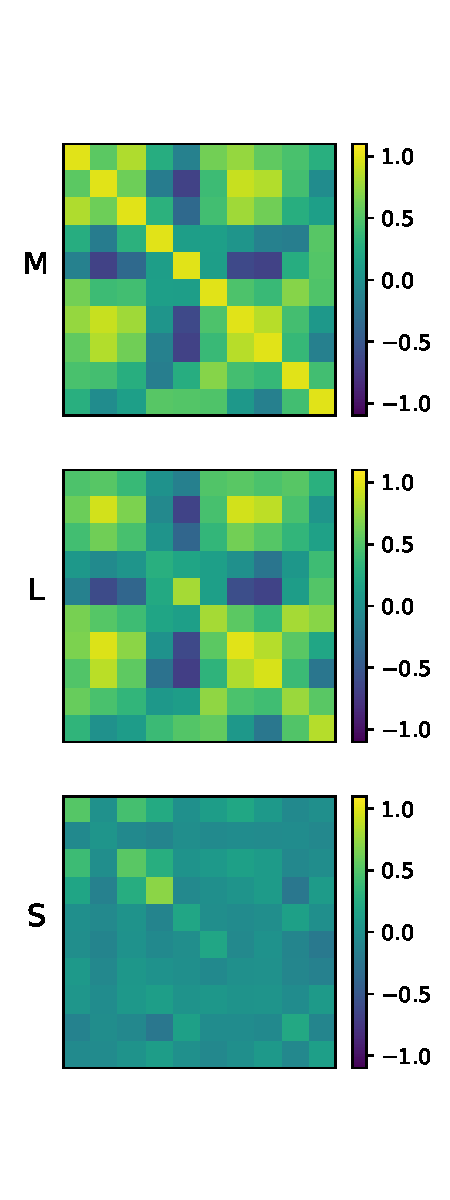
\includegraphics[width=0.48\textwidth]{fig/pcp_output_finance.pdf}
	\caption{Comparison of RPCA on the empirical $10\times 10$ covariance matrix based on the price development of 10 share certificates (see main text) from the DAX 30. The left panel shows the resulting decomposition $M=L+S$ obtained from the neural network approach, while the right panel shows the results from PCP.}
	\label{fig:compfinance}
\end{figure}


\subsection{Correlation matrix of personality features with PCP and Denise}
Here we compare the performance of the RPCA of our neural network approach and the benchmark PCP algorithm on 25 personality self report items obtained from approximately 2800 individuals. The studied 25 personality features are grouped in the five categories agreeableness, conscientiousness, extraversion, neuroticism, and openness, see \href{https://www.personality-project.org/r/html/bfi.html}[personality-project]. The aim of PCA is to recover these five underlying putative factors from the data.

In this subsection we compare the performance of PCP and our neural network approach to obtain the RPCA-decomposition of the correlation matrix of the 25 personality features. The correlations are defined as the normalized empirical covariances between the variables $x_i$
\[
M_{ij} = \text{Corr}(x_i,x_j) = \frac{\text{Cov}(x_i,x_j)}{\sqrt{\text{Var}(x_i) \text{Var}(x_i)}} \,.
\]
As in the previous subsection, we calculate the RPCA-decomposition $M=L + S$ by means of our neural network approach as well as by using the PCP method introduced in \ref{sec:pcpalgorithm}. The obtained low rank matrix $L$ and the sparse part $S$ containing corruptions of the input matrix are shown in Fig. \ref{fig:comppsych}. The low-rank ($k=10$) is determined by the PCP-algorithm, and subsequently used in the definition of the neural network. The training performance of the neural network (training and validation loss) is depicted in Fig. \ref{fig:personality_training}. The training was performed on 80000 synthetic $25\times 25$ positive semi-definite matrices of rank $10$.

As in the analysis of the financial data, the neural network decomposition exhibits very few strong outliers on the diagonal, which suppress the visual structure of the obtained matrices $L,S$ to some extend. As before, these outliers are not present in the PCP results. Hence, the PCP-method seems to function more stable than the network ansatz. We quantify the discrepancy of the resulting decomposition of both approaches by their relative distances
\begin{equation}
\epsilon_\text{rel}(S_\text{PCP},S_\text{NN}) = 3.24 \,, \quad  \epsilon_\text{rel}(L_\text{PCP},L_\text{NN}) = 2.14 \,.
\end{equation}

The comparison of both methods, in combination with the striking results reported in \cite{herrera2020denise}, may be explained by a sub-optimal choice of network-architecture (to few nodes per hidden layer) of our network. Another source of instability might result from the small training sets or not ideally chosen hyper-parameters such as batch-size. This will be analyzed in detail in future work. Moreover, we will analyze, how we can use RPCA to obtain characteristic information about the studied data. For example, it will be interesting to investigate in which way we can recover the five underlying personality categories agreeableness, conscientiousness, extraversion, neuroticism, and openness from the principal components.


\begin{figure}
	\centering
	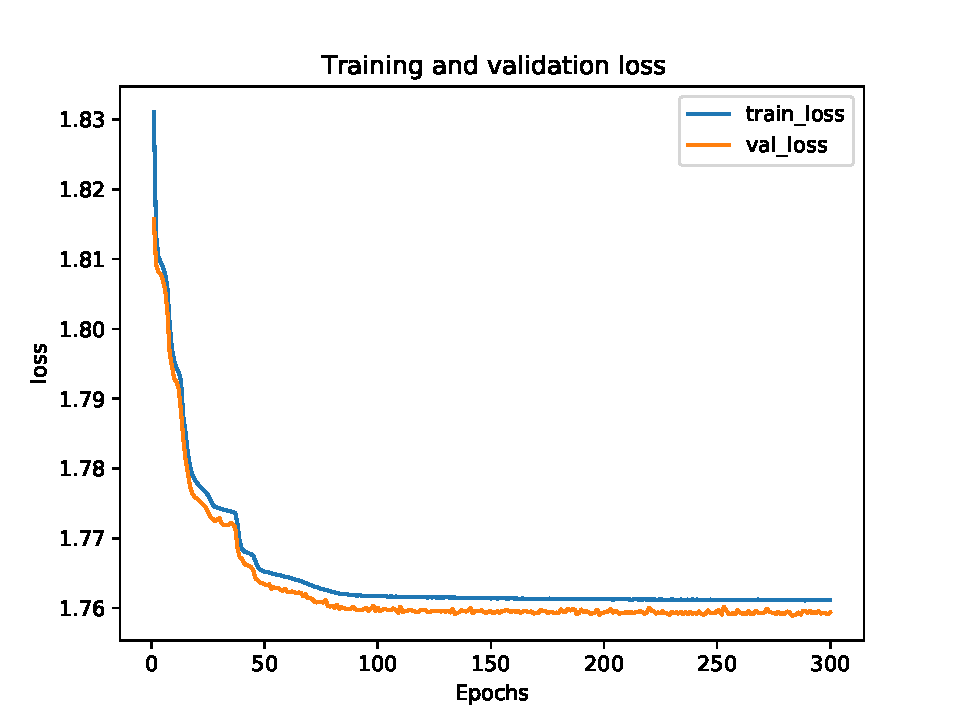
\includegraphics[width=0.6\textwidth]{fig/loss_psych.pdf}
	\caption{Training and validation loss of the training of our neural network for the personality data. Curiously, the validation loss is always smaller then the training loss.}
	\label{fig:personality_training}
\end{figure}


\begin{figure}
	\centering
	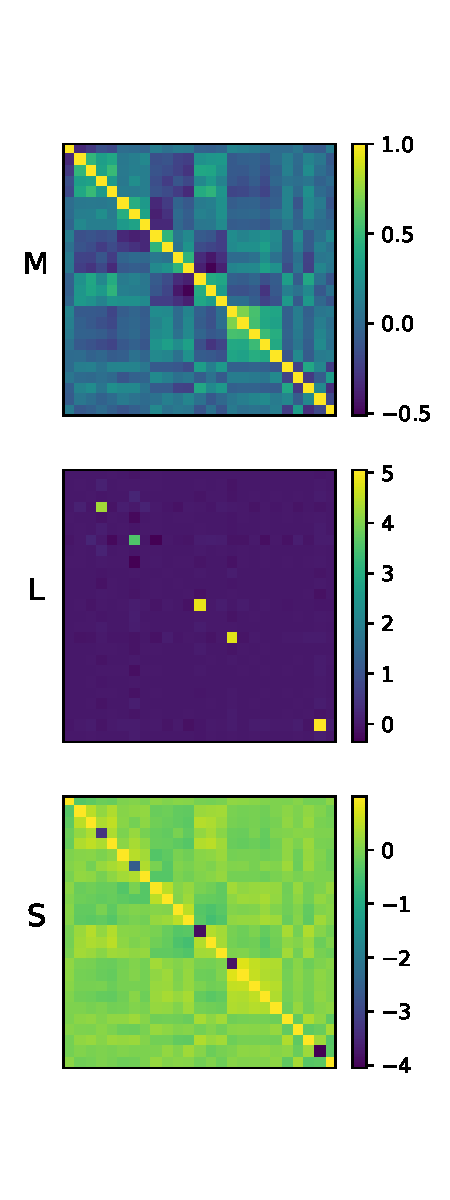
\includegraphics[width=0.48\textwidth]{fig/denise_output_psych.pdf}
	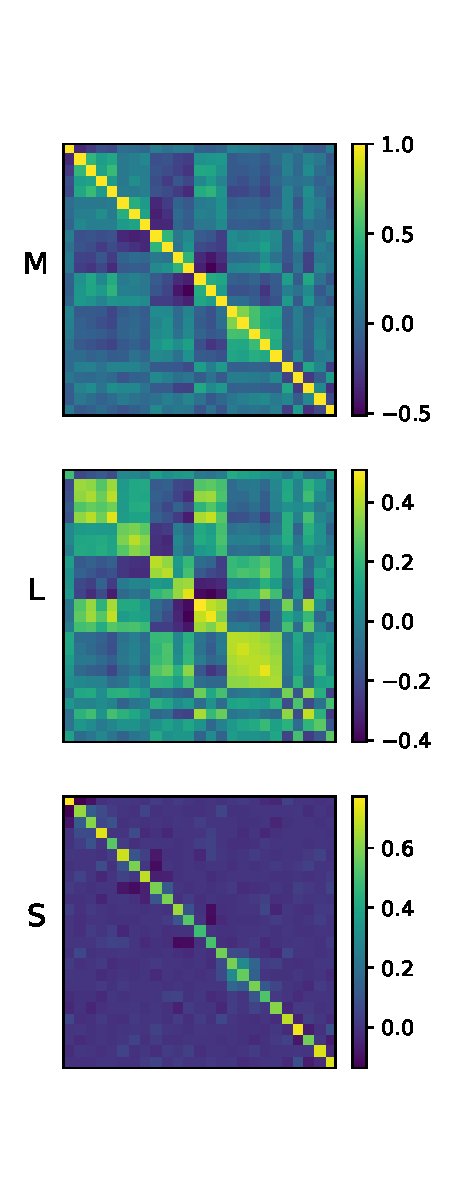
\includegraphics[width=0.48\textwidth]{fig/pcp_output_psych.pdf}
	\caption{Comparison of RPCA of the empirical $25\times 25$ covariance matrix of 27 personality features of roughly 2800 individuals (see main text). The left panel shows the resulting decomposition $M=L+S$ obtained from the neural network approach, while the right panel shows the results from PCP.}
	\label{fig:comppsych}
\end{figure}













